\documentclass[conference]{IEEEtran}
\IEEEoverridecommandlockouts

\usepackage{cite}
\usepackage{amsmath,amssymb,amsfonts}
\usepackage{algorithmic}
\usepackage{graphicx}
\usepackage{textcomp}
\usepackage{xcolor}
\usepackage{tikz}
\usetikzlibrary{arrows.meta,positioning,shapes.misc}


\title{
    CSE342: SML Course Project Report \\
    \thanks{\textit{
        CSE342: Statistical Machine Learning (Winter 2023),
        Dr Koteswar Rao Jerripothula, IIIT-Delhi.
    }}
}

\author{
    \IEEEauthorblockN{Divyajeet Singh (2021529)} \vspace*{3.0pt}
    \IEEEauthorblockA{
        \textit{Computer Science \& Engineering Dept.} \\
        \textit{IIIT-Delhi, India} \\
        divyajeet21529@iiitd.ac.in
    }
    \and
    \IEEEauthorblockN{Siddhant Rai Viksit (2021565)} \vspace*{3.0pt}
    \IEEEauthorblockA{
        \textit{Computer Science \& Engineering Dept.} \\
        \textit{IIIT-Delhi, India} \\
        siddhant21565@iiitd.ac.in
    }
}

\begin{document}
    \maketitle

    \begin{abstract}
        This report presents the findings from the course project for \textit{Statistical Machine Learning},
        held as a Kaggle contest to build a machine learning model for fruit-classification.
        The goal was to achieve the highest accuracy across a leaderboard of 50+ teams.
        A Logistic Regression model achieved the best score, attaining an accuracy of 0.82692.
    \end{abstract}

    \begin{IEEEkeywords}
        (Multi-class) Classification, Dimensionality Reduction, Anomaly Detection, Logistic Regression
    \end{IEEEkeywords}

    \section{Introduction}
    \label{sec:intro}
    This document acts as a report for the Kaggle challenge (22 Mar - 18 Apr), held as the course project for \textit{Statistical Machine Learning (Winter 2023)}.
    Given a limited dataset of 1216 images of 4096 dimensions each, the goal was to build a robust machine learning model to classify the images into one of 19 classes.
    Various approaches were discovered to tackle this multi-class classification problem.
    Appropriate advanced algorithms covered in the course were used to preprocess the data and build a classifier.

    This report provides a detailed description of the methods used, discarded, and the results obtained during the study.

    \section{Literature Review}
    \label{sec:litreview}

    \subsection{Classification (Statistical)}
    \label{sec:classification}
    Statistical classification is the problem of identifying which of a set of categories/sub-populations an observation belongs to.
    In the domain of machine learning, classification is a supervised (usually frequentist) learning technique that, given a labeled set of training data, infers a
    function to assign new examples into one or more discrete categories.

    The final submission of this project makes use of the multinomial variant of Logisitic Regression to solve the given problem.
    \vspace*{3.0pt}

    \subsubsection{Logistic Regression}
    \label{sec:lr}
    A statistical method used to analyze and model between a (usually binary) dependent variable and one or more independent variables.
    This regression analysis technique aims to predict the probability of an unseen example belonging to a particular class.

    \subsection{Dimensionality Reduction}
    \label{sec:dimred}
    Dimensionality reduction is the transformation of data from a high-dimensional space into a low-dimensional space in a way that
    retains the most meaningful and prominent properties of the original data, ideally close to its intrinsic dimension.
    Owing to the curse of dimensionality, dimensionality reduction is a common preprocessing step in machine learning.

    This project makes use of the Principal Component Analysis and Linear Discriminant Analysis algorithms for projection of features into a lower-dimensional space.
    \vspace*{3.0pt}

    \subsubsection{Principal Component Analysis (PCA)}
    \label{sec:pca}
    A statistical method that uses an orthogonal transformation to convert a set of observations of possibly correlated variables
    into a set of values of linearly uncorrelated variables called principal components.
    The first principal component accounts for the highest variability in the data, and each succeeding component has the highest possible variance under the constraint
    that it is orthogonal to all preceding components.
    \vspace*{3.0pt}

    \subsubsection{Linear Discriminant Analysis (LDA)}
    \label{sec:lda}
    A supervised statistical procedure used for dimensionality reduction by separating the features in a way that maximizes inter-class and minimizes intra-class variance.
    The resulting features are linear combinations (weighted sums) called \textit{discriminant functions} of the original features that best explain the dataset and are used to
    project the data into a lower-dimensional space.

    \subsection{Anomaly (Outlier) Detection}
    \label{sec:outlier}
    In data analysis, anomaly detection refers to the identification of observations which deviate significantly from the majority of the data and
    do not conform to a well-defined notion of normal behaviour.
    Such examples may arouse suspicions of being generated by a different mechanism, or appear inconsistent with the remainder of that dataset.

    The Local Outlier Factor procedure was used to detect outliers in the dataset.
    \vspace*{3.0pt}

    \subsubsection{Local Outlier Factor (LOF)}
    \label{sec:lof}
    A density-based statistical technique that computes the local density deviation of a given data point with respect to its neighbours to identify if it is an outlier.
    It is a measure of how isolated a data point is with respect to the surrounding neighborhood.
    The most anomalous observations are those that have a substantially lower density than their neighbours and are hence considered outliers.

    \section{Methodology}
    \label{sec:methodology}
    This section provides a detailed description of the methods used to preprocess the data and build the classifier.

    \subsection{Data Analysis and Sanity Check}
    \label{sec:dataanalysis}
    To analyze the dataset, 10 images selected at random were plotted in a 64 $times$ 64 plot, but the results were not meaningful.
    It was concluded that the features of the dataset must have been shuffled to prevent cheating in the contest by visualizing
    the data and submitting a manually labeled CSV file.

    The sanity check, hence, failed.

    \subsection{Data Preprocessing}
    \label{sec:dataprep}
    The labeled dataset provided for the challenge consisted of 1216 images of 4096 ($64 \times 64$) dimensions each.
    The images were of 19 different fruits, with each class having a different number of images.
    The data was preprocessed to increase cross-consistency using the following steps:

    \subsubsection{Outlier Detection}
    \label{sec:outlierdetection}
    It was clear that the dataset was sparse in 4096 (flattened) dimensions.
    Since it had a large number of dimensions and only a very few training samples, it was only reasonable to tune the
    Local Outlier Factor algorithm to detect only the most extreme outliers.
    This resulted in the removal of less than 16 images from the dataset.

    \begin{table}[htbp]
        \caption{Final Hyperparameters for LOF}
        \begin{center}
            \begin{tabular}{|c|c|}
                \hline
                \textbf{Hyperparameter} & \textbf{Value} \\
                \hline
                \texttt{n\_neighbors} & 10 \\
                \hline
                \texttt{contamination} & 0.01 \\
                \hline
            \end{tabular}
            \label{tab:lof}
        \end{center}
    \end{table}

    Table \ref{tab:lof} shows the final hyperparameters selected for outlier detection using LOF.

    \subsubsection{Standardization}
    \label{sec:standardization}
    Standardization is a common preprocessing step to build classifers, especially those classifying images.
    The images were standardized to have zero mean and unit variance to ensure that the features of the
    dataset were on the same scale and to prevent any feature from dominating the classifier.

    \subsubsection{Dimensionality Reduction}
    \label{sec:dimreduction}
    Owing to the sparsity of the dataset, dimensionality reduction was necessary to improve the performance of the classifier.
    The dimensionality reduction was performed using the Principal Component Analysis (PCA) and Linear Discriminant Analysis (LDA) algorithms.

    With the features of these algorithms mentioned in Section \ref{sec:dimred}, it was concluded that an LDA after a PCA would be the best choice
    to extract the features that capture the most variance in the dataset and project them onto an even lower-dimensional space to increase inter-class separation.

    \subsubsection{Train-Test Split}
    The training data was finally split in an 80:20 ratio into training and validation sets.
    The training set was used to train the classifier and the validation set was used to tune the hyperparameters of the classifier.

    \subsection{Classification Model Selection}
    \label{sec:modelselection}
    Various statistical classification techniques were covered in the course.
    However, due to the nature of the data, not all of them were suitable for the task.
    The following techniques were considered for the task:

    \subsubsection{$k$-Nearest Neighbours}
    \label{sec:knn}
    A non-parametric technique that classifies a data point based on the class of its $k$-nearest neighbours.
    The algorithm, known for its simplicity, was found to be inadequate while testing to model the complexity of the dataset.

    \subsubsection{Gradient Boosting}
    \label{sec:gb}
    A predictive modelling technique that produces a prediction model in the form of an ensemble of weak prediction models, typically decision trees,
    where each subsequent learner tries to correct the errors made by its predecessors.
    Known for its invariability to overfitting, it was one of the first algorithm tested for the task.

    However, the gradient boosting model was found to be dissatisfactory, as it was unable to generalize well on the validation set.

    \subsubsection{Random Forest}
    \label{sec:rf}
    An ensemble learning method for classification that operates by constructing a multitude of decision trees and classifies using the majority vote of the trees.
    Although the dimensionality of the dataset was reduced, the random forest model was found to be overfitting on the training set
    and was unable to perform any better than the other models.

    \subsubsection{Gaussian Naive Bayes}
    \label{sec:gnb}
    A probabilistic classifier based on Bayes' theorem with an assumption of independence between every pair of features.
    Known for its accurate performance on small datasets, an attempt was made to transform the dataset into a Gaussian distribution using the Box-Cox transformation to use it.
    However, the model was not fit for the dataset.

    \subsubsection{Neural Networks}
    \label{sec:nn}
    A model having interconnected layers of mathematical functions (neurons) to apply activation functions on inputs from the previous layers to produce subsequent outputs.
    The neural network was found to be one of the most suitable models for the task, as it was able to learn well on the limited dataset available.

    Surprisingly, the score of the neural network model dropped down when the full testing dataset was used.
    Hence, the model was not used for the final submission.

    \subsubsection{Multinomial Logistic Regression}
    (Described in Section \ref{sec:lr}) \\
    An extension of logistic regression performed substantially better than all other models, except for the neural network, which
    was a close second.
    It performed well on multiple trials, each involving a different subset as the training set and the validation set.
    This model was also able to generalize well on the testing dataset.

    \subsection{Hyperparameter Tuning}
    \label{sec:hyperparam}
    Having finally decided on a pipeline, the validation set was used to tune the hyperparameters of the classifier.
    A grid search was performed to exhaustively search for the optimal hyperparameters for the different steps of the final model.

    A pipeline was constructed having PCA, LDA, and Logistic Regression as the steps.
    Invariably, they were tested with different lists of hyperparameters and cross validated using $k$-fold cross validation technique.
    The grid search returned the following hyperparameters for the final model:

    \begin{table}[htbp]
        \caption{Final Hyperparameters found by Grid Search}
        \begin{center}
            \begin{tabular}{|c|c|c|}
                \hline
                \textbf{Algorithm} & \textbf{Hyperparameter} & \textbf{Value} \\
                \hline
                PCA & \texttt{n\_components} & 256 \\
                \hline
                LDA & \texttt{n\_components} & 18 \\
                \hline
                 & \texttt{max\_iter} & 10,000 \\
                \cline{2-3}
                Logistic Regression & \texttt{C} & 0.1 \\
                \cline{2-3}
                & \texttt{solver} & sag \\
                \hline
            \end{tabular}
            \label{tab:hyperparams}
        \end{center}
    \end{table}

    Table \ref{tab:hyperparams} shows the final hyperparameters selected for the final model.
    The results from the grid search were obtained after 5-fold cross validation on each combination of possible hyperparameters.
    The hyperparameters were selected based on the highest average accuracy obtained on the validation set.

    \section{The Final Model}
    \label{sec:finalmodel}
    The inferred hyperparameters for all algorithms were used to train the final model on the entire dataset.
    The model was trained using a pipeline, which was then used to predict the labels of the testing dataset. \\
    \vspace*{10pt}

    \begin{figure}[htbp]
        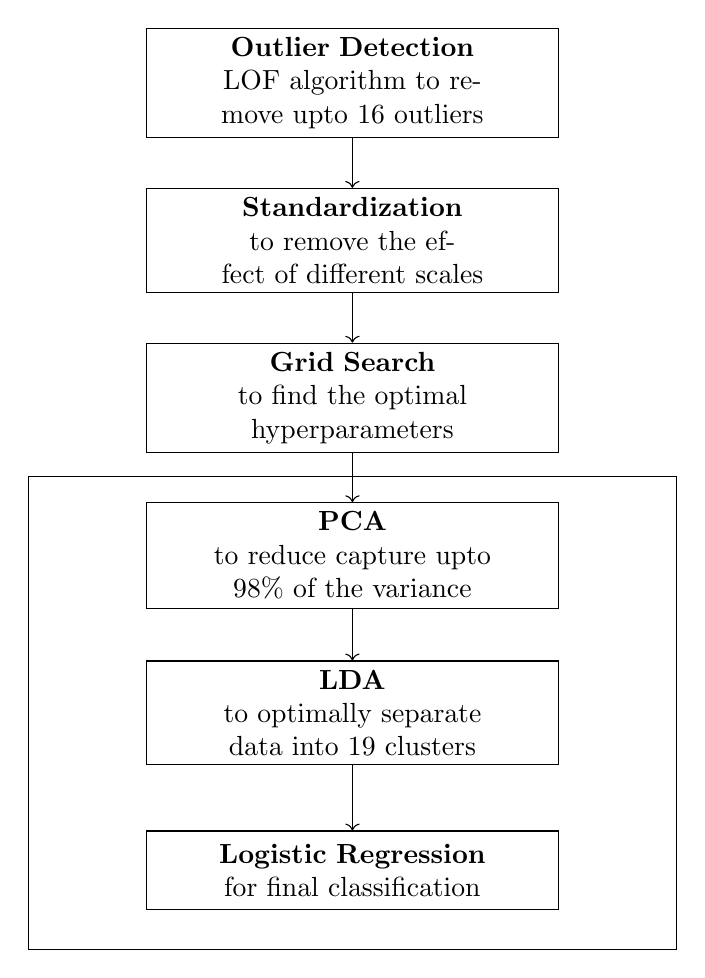
\begin{tikzpicture}[node distance=2cm]
            \node (a) [rectangle, draw, text width=5cm, minimum height=1cm, text centered] {\textbf{Outlier Detection} \\ LOF algorithm to remove upto 16 outliers};
            \node (b) [rectangle, draw, text width=5cm, minimum height=1cm, text centered, below of=a] {\textbf{Standardization} \\ to remove the effect of different scales};
            \node (c) [rectangle, draw, text width=5cm, minimum height=1cm, text centered, below of=b] {\textbf{Grid Search} \\ to find the optimal hyperparameters};
            \node (e) [rectangle, draw, text width=5cm, minimum height=1cm, text centered, below of=c] {\textbf{PCA} \\ to reduce capture upto 98\% of the variance};
            \node (f) [rectangle, draw, text width=5cm, minimum height=1cm, text centered, below of=e] {\textbf{LDA} \\ to optimally separate data into 19 clusters};
            \node (d) [rectangle, draw, text width=8cm, minimum height=6cm, text centered, below of=e] {};
            \node (g) [rectangle, draw, text width=5cm, minimum height=1cm, text centered, below of=f] {\textbf{Logistic Regression} \\ for final classification};

            \draw [->] (a) -- (b);
            \draw [->] (b) -- (c);
            \draw [->] (c) -- (e);
            \draw [->] (e) -- (f);
            \draw [->] (f) -- (g);
            \label{fig:finalmodel}
        \end{tikzpicture}
        \caption{Pipeline used for the final model}
    \end{figure}

    Fig. 1 shows the flow of final model used for the classification, including all the steps performed on the dataset.
    The steps included in the enclosing box indicate the final pipeline.

    \section{Conclusion}
    \label{sec:results}
    A CSV file following the given format was generated as the prediction from the pipeline and submitted to the Kaggle competition for evaluation.
    The final model was able to achieve a score of 0.82692 on the testing dataset, leading to a rank of 5 out of 57 teams on the leaderboard.

    \section*{Acknowledgment}
    \label{sec:acknowledgment}
    The authors would like to extend their sincerest gratitude to Dr Koteswar Rao Jerripothula
    \textit{(Computer Science \& Engineering Dept., IIIT-Delhi)} for their invaluable guidance throughout the project.
    Their insightful feedback and expertise have been instrumental in shaping this project into its final form.

    The authors would also like to thank Niranjan Sundararajan (2020090), Vibhu Dubey (2020150), and Raghav Sahni (2020533),
    the teaching assistants of the course \textit{Statistical Machine Learning (Winter 2023)}, for their unwavering support.

    \begin{thebibliography}{00}
        \bibitem{b1} Dr Koteswar Rao Jerripothula, lecture notes, Statistical Machine Learning (Winter 2023), IIIT-Delhi.
        \bibitem{b2} sklearn, \underline{https://scikit-learn.org/stable/}
    \end{thebibliography}
\end{document}